%------------------------------------------------
% Quick reference. 
%------------------------------------------------
%
% Для вставки картинок:
%
%--------         Комманда
%
%\begin{figure}[H]
%	\includegraphics{img_name}
%	\caption{some caption}
%	\label{some_pic}
%\end{figure}
%
%--------        Переменные
%
% img_name     <- Название картинки в папке img.
% some_caption <- подпись картинки.
% label        <- лейбл нужен для ссылок на картинку.
% H            <- расположение картинки на странице.
%
%--------         Пример
%
%\begin{figure}[H]
%	\includegraphics{pic1.jpg}
%	\caption{График}
%	\label{grapics1}
%\end{figure}
%
%------------------------------------------------
%
% Для референса по лейблу:
%
%--------         Комманда
%
% Для ссылки используется \eqref{ref}.
%
%--------        Переменные
%
% ref          <- указанный лейбл в директиве \label{ref}
%                 Ссылку можно сделать на любой объект имеющий \label{•}
%
%--------         Пример
%
% \eqref{graphics1}
%
%------------------------------------------------
%
% Для листинга кода:
%
%--------         Комманда
%
% \lstinputlisting[language=lang,mathescape=true]{src}
%--------        Переменные
%
% lang         <- язык на котором написан исходный код, например "python" или "C++".
% mathescape   <- если в исходниках есть формулы LaTeX, то они будут представлены как формулы.
% src          <- путь до файла исходников.
%
%--------         Пример
%
% \lstinputlisting[language=C++,mathescape=false]{./src/main.cpp}
%
%------------------------------------------------
%
% Для вставки таблиц:
%
%--------
%\begin{table}[H]
%	\centering
%	\caption{ capt }
%	\begin{tabularx}{0.9\textwidth}{ | Y | Y | }
%		\hline
%		lines
%	\end{tabularx}
%	\label{tab1}
%\end{table}
%--------
% caption      <- Подпись таблицы.
% tab1         <- лейбл нужный для ссылки на таблицу.
% | Y | Y |    <- количество и формат столбцов.
% Y            <- Тип столбца.
%                 В данном случае определены кастомные столбцы Y (Спасибо Максиму Наумову)
% |            <- обозначает границы столбца.
%                 То есть, если будет указано |Y Y|, то столбцы внутри строк разделены не будут.
% H            <- То же самое, что и у картинок.
% lines        <- непосредственно элементы таблицы.
%                 Разделяются знаком "&", оканчивать каждую строку лучше \\ \hline
%
%--------         Пример
%\begin{table}[H]
%	\centering
%	\caption{ capt }
%	\begin{tabularx}{0.9\textwidth}{ | Y | Y | }
%		\hline
%		str1 & str2 \\ \hline
%		str1 & str2 \\ \hline
%		str1 & str2 \\ \hline
%		str1 & str2 \\ \hline
%		str1 & str2 \\ \hline
%	\end{tabularx}
%	\label{tab1}
%\end{table}
%------------------------------------------------

\documentclass[12pt, fleqn, a4paper]{extarticle}

\makeatletter
\renewcommand*\l@section{\@dottedtocline{1}{1.5em}{2.3em}}



%\includegraphics{universe}

\usepackage[utf8]{inputenc}
\usepackage[T2A]{fontenc}
\usepackage[russian]{babel} % указывает язык документа
\usepackage[left=3cm,right=2cm,top=2cm,bottom=2cm,bindingoffset=0cm]{geometry}
\usepackage{lastpage}
\usepackage[none]{hyphenat}
\usepackage{fancyhdr}
\usepackage{titlesec}
\usepackage{graphicx} % для вставки картинок
\usepackage[intlimits]{mathtools} % математические дополнения
\usepackage{amssymb}
\usepackage[tableposition=top]{caption}
\usepackage{subcaption}
\usepackage{indentfirst}
%\usepackage{minted}
\usepackage{listings}
\usepackage{tabularx}
\usepackage{tabulary}
\usepackage{multirow}
\usepackage{float}
\usepackage[figure,table]{totalcount}
\usepackage{diagbox}
\usepackage[german=guillemets]{csquotes}
\usepackage{fontspec} 
\usepackage{enumitem}
%\usepackage{mathptmx}% http://ctan.org/pkg/mathptmx
%\usepackage{showframe}
\usepackage{hyperref}

\setlength{\parindent}{1.2cm}

\setlength{\mathindent}{1.2cm}

\defaultfontfeatures{Ligatures={TeX},Renderer=Basic} 
\setmainfont[Ligatures={TeX,Historic}]{Times New Roman}

%\setlist[enumerate]{itemindent=\dimexpr\labelwidth+\labelsep\relax,leftmargin=0pt}

%\setlength{\section*}{0.5cm}
%\usepackage{minted}
%\usepackage{fancyvrb}
%\usepackage{newtxtext}

%\titleformat{\section}[hang]{\bfseries\LARGE\centering}{}{1em}{}

%\setlist[enumerate]{itemindent=\dimexpr\labelwidth+\labelsep\relax,leftmargin=0pt}
\setlist[enumerate,itemize]{leftmargin=0pt,itemindent=1.7cm}

\titleformat{\section}{\large\bfseries\centering}{\thesection}{0.5em}{\MakeUppercase}
\titleformat{\subsection}[block]{\bfseries\hspace{1em}}{\thesubsection}{0.5em}{}
%\setlength{\subsection*}{1.5cm}
%\setlength{\parindent}{4em}

%\setlength{\parindent}{1.5cm}

\captionsetup[figure]{labelfont={it},textfont={it},name={Рисунок},labelsep=endash, skip=5pt}
\captionsetup[table]{labelfont={it},textfont={it},name={Таблица},labelsep=endash,singlelinecheck=false, skip=5pt, margin=1cm}

\lstset{
	basicstyle=\footnotesize\ttfamily,
	columns=fullflexible,
	keywordstyle=\color{blue},
	%frame=single,
	breaklines=true,
	numberstyle=\tiny\color{mygray},
	postbreak=\mbox{\textcolor{red}{$\hookrightarrow$}\space},
	showstringspaces=false,
}

%\renewcommand{\baselinestretch}{1.5}
\linespread{1.5} % полуторный интервал
\frenchspacing
\graphicspath{ {images/} }

  %-------------------------------------------
  % Переменные
  %-------------------------------------------

  \newcommand{\firstAuthorSurName}{Белоусов} 					                           % Фамилия автора.
  \newcommand{\firstAuthorInitials}{ А. А.} 					                           % Фамилия автора.
  % \newcommand{\leftcolon}{Уравнения Математической Физики}
  %\newcommand{\secondAuthorSurName}{Родин} 					                           % Фамилия автора.
 % \newcommand{\secondAuthorInitials}{ И. А.} 					                           % Фамилия автора.
  \newcommand{\teacherName}{Кириленко М.С.}				                               % Имя преподавателя.
%  \newcommand{\variantNumber}{25} 							                           % Номер варианта.
  \newcommand{\groupNumber}{6409-010302D} 				                               % Номер группы.
  %\newcommand{\subjectTitle}{Отчет по лабораторной работе No1}                                  % Название предмета.
%  \newcommand{\taskTitle}{Дисциплина \enquote{Уравнения математической физики}} 		  % Название работы.
%  \newcommand{\theme}{АНАЛИТИЧЕСКОЕ РЕШЕНИЕ КРАЕВЫХ ЗАДАЧ МАТЕМАТИЧЕСКОЙ ФИЗИКИ} 		  % Название работы.
  
  %-------------------------------------------
  % Ссылки в оглавлении
  %-------------------------------------------
  

\hypersetup{
    colorlinks,
    citecolor=black,
    filecolor=black,
    linkcolor=black,
    urlcolor=black
}

  %-------------------------------------------
  % Стиль футеров и хедеров
  %-------------------------------------------

\pagestyle{fancy}
\fancyhead[L, R]{}
\fancyfoot[L]{}
\fancyfoot[R]{}
\renewcommand{\footrulewidth}{0pt}
\renewcommand{\headrulewidth}{0pt}

%\renewcommand\subsectionfont{\normalfont\normalsize\bfseries}

\def\l@subsection{\@dottedtocline{2}{3.8em}{3.2em}}

\newcolumntype{Y}{>{\centering\arraybackslash}X}

\begin{document}

%----------------------------------------------------------------------------------------
%	TITLE PAGE
%----------------------------------------------------------------------------------------
\pagenumbering{Alph}

\begin{titlepage}
							
	\center
							
	%------------------------------------------------
	%	Заголовки
	%------------------------------------------------
							
	\textsc{Министерство образования и науки Российской Федерации}\\[-0.15cm]
	\textsc{Федеральное государственное автономное образовательное учреждение \\[-0.15cm] высшего образования}\\[-0.15cm] 
	\textsc{«Самарский национальный исследовательский университет \\[-0.15cm] имени академика С.П.Королёва»}\\[0.5cm]
	\textsc{Институт информатики, математики и электроники}\\[-0.7em]
	\textsc{Факультет информатики}\\[-0.7em]
	\textsc{Кафедра технической кибернетики}\\[-1em]
						
	%------------------------------------------------
	%	Название работы
	%------------------------------------------------
							
	\vfill\vfill
						    
							
	{\textbf{Отчет по лабораторной работе No1}}\\[-0.7em]
	{\textbf{по курсу «Оптоинформационные технологии и системы»}}
	
    \vfill\vfill\vfill\vfill\vfill\vfill\vfill\vfill\vfill
							
	\begin{minipage}{1\textwidth}
		\begin{center}
			\begin{tabularx}{\textwidth}{X l}
				Выполнил студент:        & \firstAuthorSurName \firstAuthorInitials \\
				Группа:                    & 6409                     		           \\
				Преподаватель:                  & \teacherName         		                \\
			\end{tabularx}
		\end{center}
	\end{minipage}
							
						
	%------------------------------------------------
	%	Дата
	%------------------------------------------------
							
	\vfill\vfill\vfill
					
	{\centering Самара \the\year}
							
							
\end{titlepage}

\pagenumbering{arabic}

\setcounter{page}{2}


%------------------------------------------------
%Задание
%------------------------------------------------

\section*{Задание}
{
	\begin{enumerate}
	    \item Требуется создать программу, выполняющую расчет пересечения луча с заданными поверхностями. Результатом работы программы должны быть координаты точки пересечения луча с поверхностью. В качестве поверхности выбрать плоскость, сферу и эллипсоид.
	    
        \item Дополнить программу, чтобы среди результатов были параметры луча, отраженного данной поверхностью.
        
        \item Дополнить программу, чтобы среди результатов были параметры луча, преломленного данной поверхностью.
        
        \item Создать механизм отображения хода лучей и поверхности в двумерном случае.
	\end{enumerate}
}
\newpage

%------------------------------------------------
% Начало основной части
%------------------------------------------------
\titleformat{\section}{\large\bfseries}{\thesection}{0.5em}{}
\titlespacing*{\section}{\parindent}{1ex}{1em}

\section{Описание луча}
{
	Луч задан параметрически в виде:
	\begin{equation}\label{ray_eq}
	\vec{r} = \vec{p_0} + \vec{e} t,
	\end{equation}
	где $\vec{p_0}$ -- радиус-вектор точки начала луча, $\vec{e}$ -- вектор направления луча, $t$ -- длина луча.
}

\section{Пересечение с плоскостью}
{
	Уравнение плоскости записывается в виде:
	\begin{equation}\label{plane_eq}
	(\vec{n},\, \vec{r} - \vec{r_0}) = 0,
	\end{equation}
	где $\vec{n}$ -- вектор нормали плоскости, $vec{r_0}$ -- радиус-вектор точки, через которую проходит плоскость.
	
	Формулу для длины луча получим подстановкой \eqref{ray_eq} в \eqref{plane_eq}:
	\begin{equation}\label{ray_plane_distance}
	t = \frac{(\vec{n},\, \vec{r} - \vec{p_0})}{(\vec{n},\, \vec{e})}.
	\end{equation}
	
	Используем для расчета следующие параметры луча и плоскости:
	\begin{enumerate}
	\item Параметры луча: $\vec{p_0} = (0, 0)$, $\vec{e} = (1, 2)$;
	\item Параметры плоскости: $\vec{n} = (1, 0)$, $\vec{r_0} = (3, 2)$.
	\end{enumerate}
	
	Получим точку пересечения луча с плоскостью: $(3, 6)$.
	
	Длина луча до точки пересечения: $t = 1.044$.
	
	На рисунках \ref{plane_intersect1}-\ref{plane_intersect3} представлены результаты пересечения луча и плоскости при различных значениях коэффициентов преломления $n_1$, $n_2$.

	\begin{figure}[H]
		\centering
		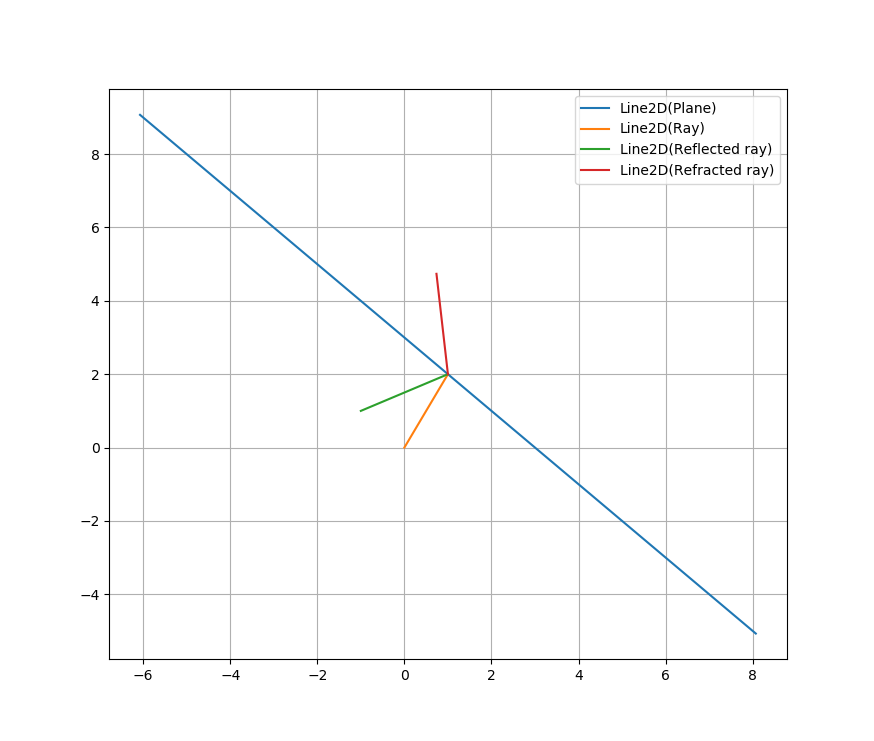
\includegraphics[width=0.65\pagewidth]{plane_intersect1}
		\caption{Пересечение с плоскостью при $n_1 = 1$, $n_2 = 2$}
		\label{plane_intersect1}
	\end{figure}
	
	\begin{figure}[H]
		\centering
		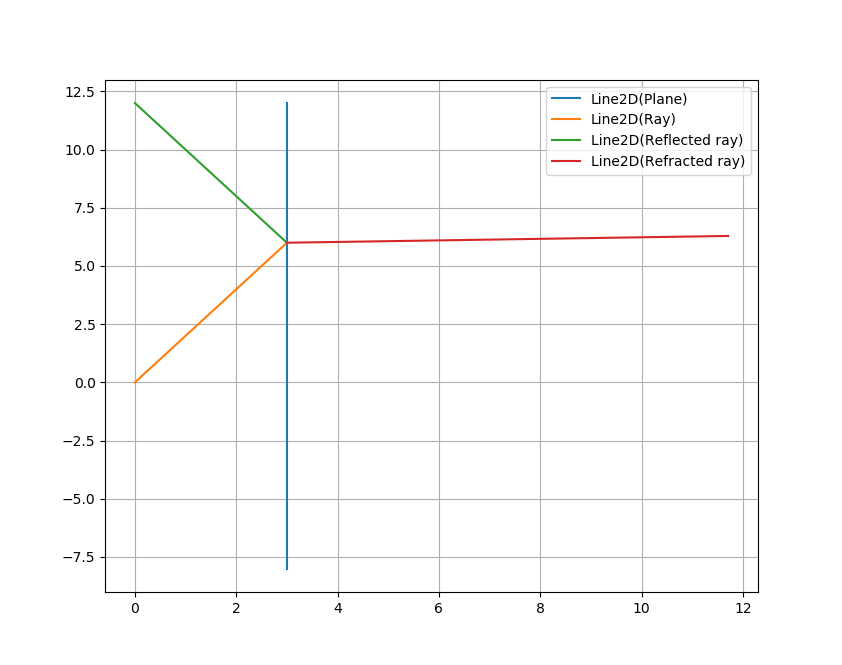
\includegraphics[width=0.65\pagewidth]{plane_intersect2}
		\caption{Пересечение с плоскостью при $n_1 = 0.1$, $n_2 = 2$}
		\label{plane_intersect2}
	\end{figure}
	
	\begin{figure}[H]
		\centering
		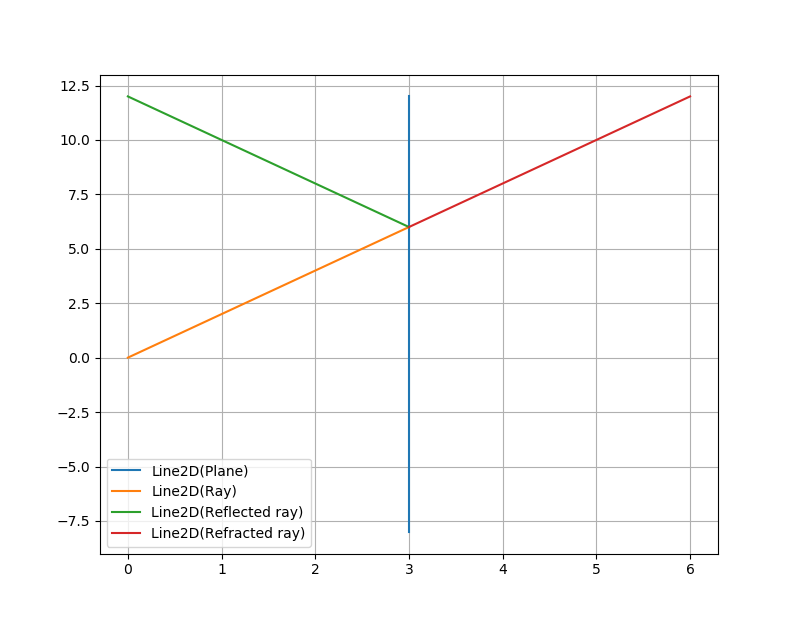
\includegraphics[width=0.65\pagewidth]{plane_intersect3}
		\caption{Пересечение с плоскостью при $n_1 = 0.5$, $n_2 = 0.5$}
		\label{plane_intersect3}
	\end{figure}
}

\newpage

\section{Пересечение луча со сферой}
{
	Сфера задаётся следующим уравнением:
	\begin{equation}\label{sph_eq}
		(\vec{p} - \vec{p_0},\, \vec{p} - \vec{p_0}) = R^2,
	\end{equation}
	где $\vec{p_0}$ -- радиус-вектор точки цетра сферы, $R$ -- радиус сферы.
	
	Формулу для длины луча получим подстановкой \eqref{ray_eq} в \eqref{sph_eq}:
	\begin{equation}\label{ray_sphere_intersect}
	t_{1,2} = (\vec{r_0} - \vec{p_0}, \vec{e}) \pm \sqrt{(\vec{r_0} - \vec{p_0}, \vec{e})^2 - (\vec{r_0} - \vec{p_0}, \vec{r_0} - \vec{p_0}) - R^2}.
	\end{equation}
	
	Луч пересекается со сферой только в следующем случае:
	\begin{equation}\label{sph_intersect_criteria}
	(\vec{r_0} - \vec{p_0}, \vec{e})^2 - (\vec{r_0} - \vec{p_0}, \vec{r_0} - \vec{p_0}) - R^2 \geq 0.
	\end{equation}
	
	Если луч пересекает сферу, то для нормали в точках пересечения имеем два варианта:
	\begin{equation}\label{sph_normal}
	\vec{n} = \frac{\vec{r(t_{1,2})} - \vec{p_0}}{||\vec{r(t_{1,2})} - \vec{p_0}||}
	\end{equation}
	
	Если поверхность выпуклая, то $(\vec{n}, \vec{e}) > 0$, если вогнутая, то $(\vec{n}, \vec{e}) < 0$.
	
	Используем для расчета следующие параметры луча и сферы:
	\begin{enumerate}
	\item Параметры луча: $\vec{p_0} = (-1, -1)$, $\vec{e} = (1, 2)$;
	\item Параметры сферы: $\vec{p_0} = (1, 1)$, $R = 2$.
	\end{enumerate}
	
	Получим точки пересечения луча со сферой: $(-0.6, -0.2)$, $(1, 3)$.
	
	Расстояния до пересечения с ближней и дальней сторонами сферы: ${t_0 = 1.2, t_1 = 5.99}$.
	
	На рисунках \ref{sph_intersect1}-\ref{sph_intersect2} представлены результаты пересечения луча и сферы при различных значениях коэффициентов преломления $n_1$, $n_2$.
	
	\begin{figure}[H]
		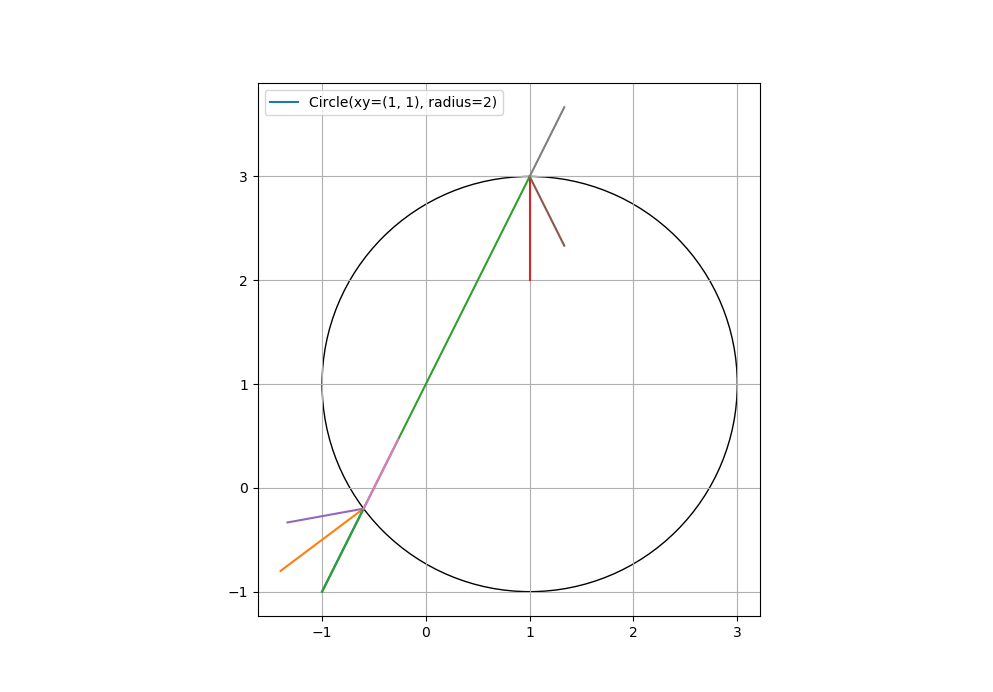
\includegraphics[width=0.7\pagewidth]{sph_intersect1}
		\centering
		\caption{Пересечение со сферой при $n_1 = 0.1$, $n_2 = 0.1$}
		\label{sph_intersect1}
	\end{figure}
	
	\begin{figure}[H]
		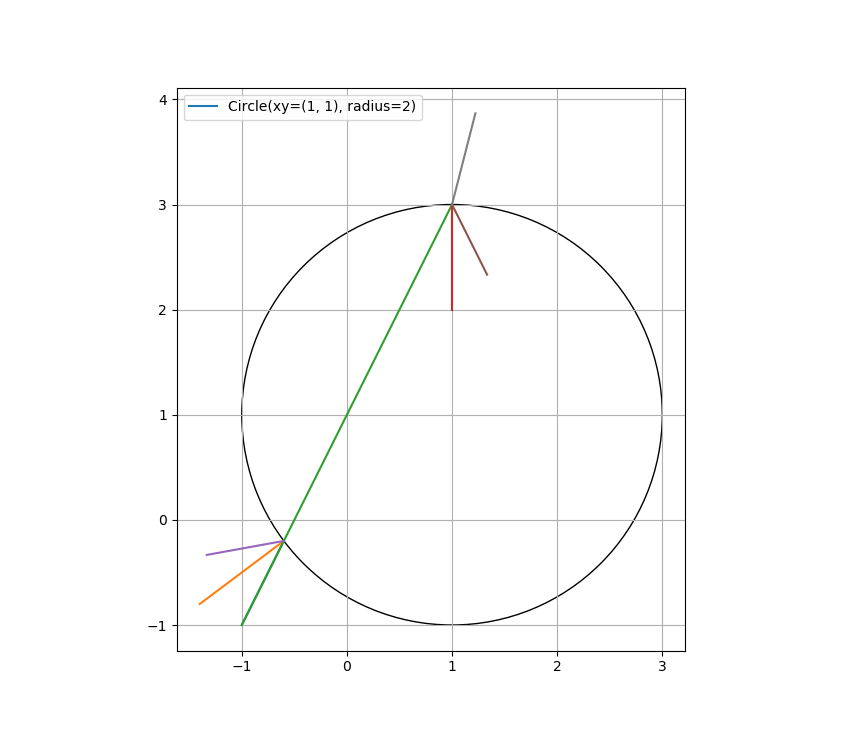
\includegraphics[width=0.7\pagewidth]{sph_intersect2}
		\centering
		\caption{Пересечение со сферой при $n_1 = 1.5$, $n_2 = 1$}
		\label{sph_intersect2}
	\end{figure}
	
%	Изменим параметры, переместив луч:
%	\begin{enumerate}
%	\item Параметры луча: $\vec{p_0} = (2, 0)$, $\vec{e} = (1, 2)$;
%	\item Параметры сферы: $\vec{p_0} = (3, 0)$, $R = 2.7$.
%	\end{enumerate}
%	
%	Координаты точки пересечения луча со сферой: $(3.34, 2.68)$.
%	
%	Длина луча: $t = 2.99$.
%	
%	Результаты представлены на рисунках \ref{sph_intersect3}-\ref{sph_intersect4}.
%	
%	\begin{figure}[H]
%		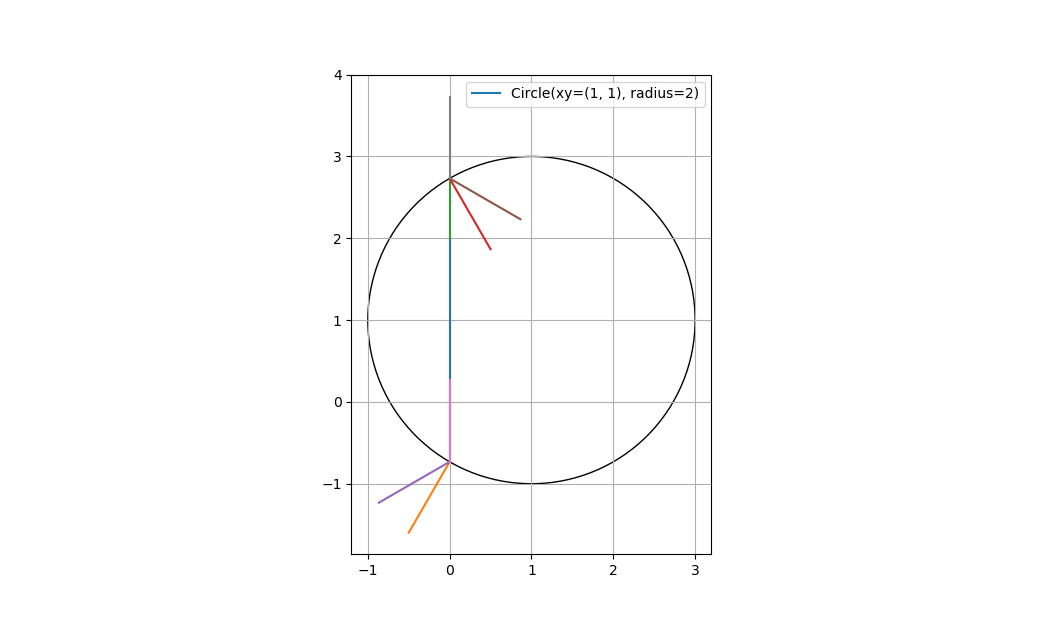
\includegraphics[width=0.7\pagewidth]{sph_intersect3}
%		\caption{Ход лучей, при $n_1 = 1$, $n_2 = 1.5$}
%		\label{sph_intersect3}
%	\end{figure}
%	
%	\begin{figure}[H]
%		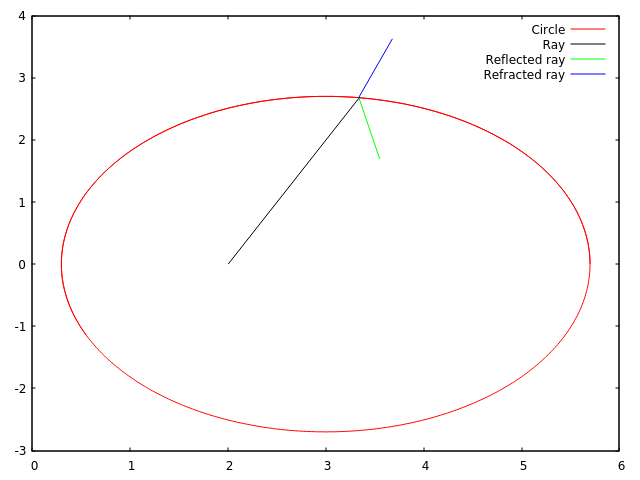
\includegraphics[width=0.7\pagewidth]{sph_intersect4}
%		\caption{Ход лучей, при $n_1 = 1.5$, $n_2 = 1$}
%		\label{sph_intersect4}
%	\end{figure}
}

\newpage

\section{Пересечение луча с эллипсоидом}{
	Эллипс задаётся следующим уравнением:
	\begin{equation}\label{ell_eq}
		\frac{(x - p_x)^2}{a^2} + \frac{(y - p_y)^2}{b^2} = 1.
	\end{equation}
	где $(p_x, p_y)$ -- радиус-вектор точки центра эллипса; $a$, $b$ -- длины полуосей эллипса.
	
	Подставив \eqref{ray_eq} в \eqref{ell_eq}, получаем квадратное уравнение относительно длины луча. 
	%Решение данного уравнения представленно в приложении А в функции \textit{intersect} соотсвествующей структуре \textit{Ellipse}.
	
	Используем для расчета следующие параметры луча и эллипсоида:
	\begin{enumerate}
	\item Параметры луча: $\vec{p_0} = (-1, -1)$, $\vec{e} = (1, 2)$;
	\item Параметры эллипса: $\vec{p_0} = (2, 2)$, $a = 4$, $b = 2$.
	\end{enumerate}
	
	Получим точки пересечения луча с эллипсом: $(-0.31, 0.36)$, $(1.49, 3.98)$.
	
	Расстояния до пересечения с ближней и дальней сторонами эллипса: ${t_0 = 2.053, t_1 = 7.476}$.
		
	Результаты представлены на рисунках \ref{ell_intersect1}-\ref{ell_intersect2}.
	
	\begin{figure}[H]
		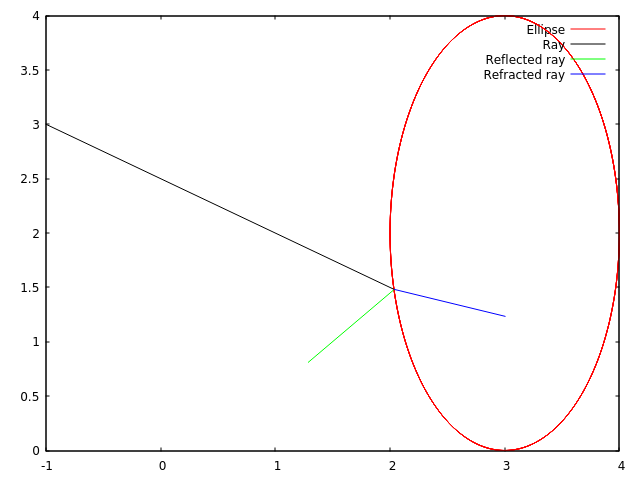
\includegraphics[width=0.7\pagewidth]{ell_intersect1}
		\caption{Пересечение с эллипсом при $n_1 = 1$, $n_2 = 1.5$}
		\label{ell_intersect1}
	\end{figure}
	
	\begin{figure}[H]
		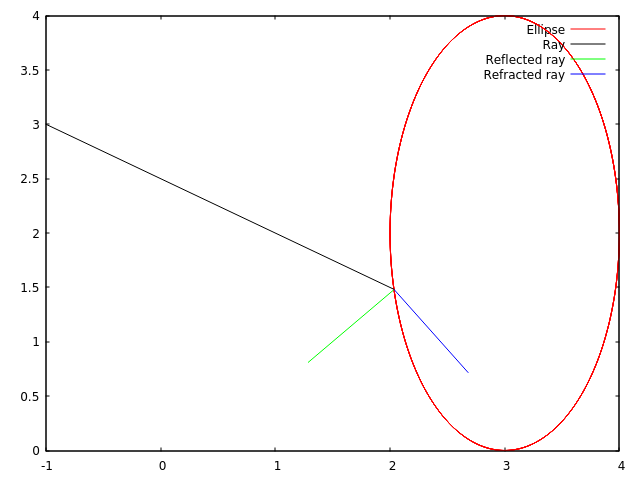
\includegraphics[width=0.7\pagewidth]{ell_intersect2}
		\caption{Пересечение с эллипсом при $n_1 = 1$, $n_2 = 1.5$}
		\label{ell_intersect2}
	\end{figure}
	
%	Для эксперимента возьмём следующие значения:
%	\begin{enumerate}
%	\item Параметры луча: $\vec{p_0} = (3.3, 1.2)$, $\vec{e} = (1, -0.2)$;
%	\item Параметры эллипса: $\vec{p_0} = (3, 2)$, $a = 1$, $b = 1.5$.
%	\end{enumerate}
%	
%	Координаты точки пересечения луча со сферой: $(3.8, 1.1)$.
%	
%	Длина луча: $t = 0.51$.
%	
%	Результаты представлены на рисунках \ref{ell_intersect3}-\ref{ell_intersect4}.
%	
%	\begin{figure}[H]
%		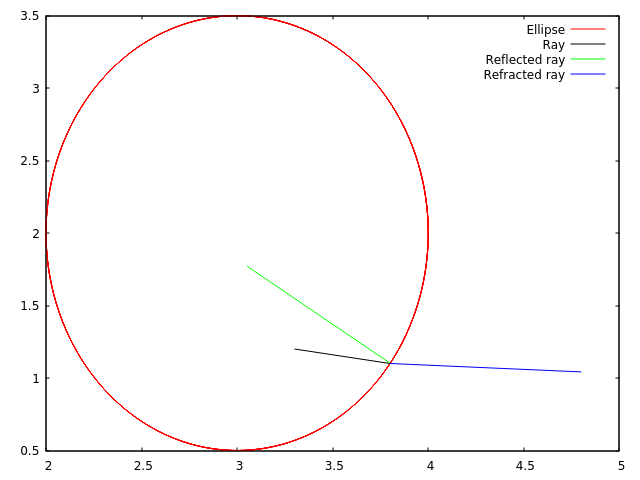
\includegraphics[width=0.7\pagewidth]{ell_intersect3}
%		\caption{Ход лучей, при $n_1 = 1$, $n_2 = 1.5$}
%		\label{ell_intersect3}
%	\end{figure}
%	
%	\begin{figure}[H]
%		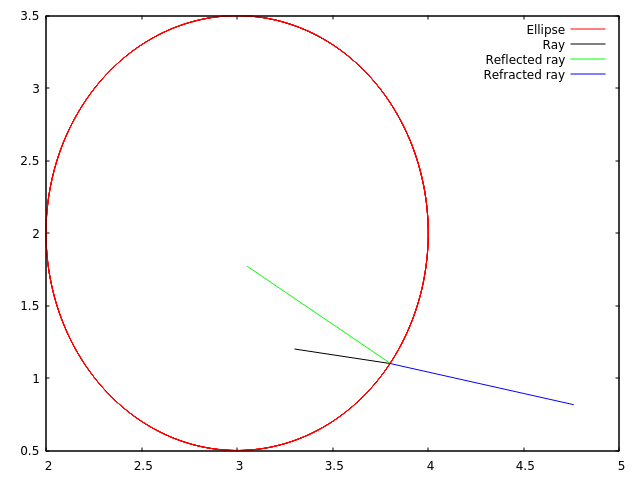
\includegraphics[width=0.7\pagewidth]{ell_intersect4}
%		\caption{Ход лучей, при $n_1 = 1.5$, $n_2 = 1$}
%		\label{ell_intersect4}
%	\end{figure}
}

\newpage

\titleformat{\section}{\large\bfseries\centering}{\thesection}{0.5em}{\MakeUppercase}
\titleformat{\subsection}[block]{\bfseries\hspace{1em}}{\thesubsection}{0.5em}{}

\section*{Заключение}{
	В данной лабораторной работе была создана программа, которая запрашивает параметры луча и параметры поверхности. Результатом работы программы являлись координаты точки пересечения луча с поверхностью. В качестве поверхности были выбраны плоскость, сфера и эллипсоид. Также был реализован механизм отображения хода лучей и поверхности в двумерном случае. Программа может отображать падающий, отраженный и преломленный лучи. Были построенные соответствующие графики хода лучей из сред с разными коэффициентами преломления. С помощью данной программы легко увидеть, как луч проходит через разные поверхности, что угол падения меньше угла преломления при переходе луча из оптически более плотной среды в оптически менее плотную. Также можно увидеть, что в зависимости от поверхности луч отражается по разному.
}

\newpage

%------------------------------------------------
% Приложения. Коды программ и.т.д.
%------------------------------------------------

\section*{Приложение А}
{
\addcontentsline{toc}{section}{Приложение А Код программы}
	\begin{center}
	\textbf{Код программы}
	\end{center}
	%\inputminted[breaklines, mathescape, fontsize=\footnotesize]{rust}{./src/main.rs}
	\lstinputlisting[language=python,mathescape=true]{./src/main.py}
}

\end{document}
